\section{运动方程计算结果}
本论文前面章节的数值计算,分别从谱函数以及序参量的角度研究了2D拓扑绝缘体/$d$-波超导体异质结系统中由近邻效应诱导产生超导配对,从而发现拓扑绝缘体中的$\mathcal{C}_4$对称性受到了破坏,而且马约拉纳束缚态也只是出现在系统的部分角落中。这里我们通过解析的方式来研究系统哈密顿量所对应的谱函数以及超导序参量在层间耦合作用下的具体表达形式,来分析引起对称性破坏的起源。
%\setcounter{page}{1}
%\pagestyle{plain}
\subsection{动量空间中的反常格林函数}
对于2D拓扑绝缘体,其轨道$\tau$的有效配对可以由反常格林函数$F_\tau(\mathbf{k},\omega)=\langle\langle c^\dagger_{\mathbf{k}\tau\uparrow}|c^\dagger_{\mathbf{-k}\tau\downarrow}\rangle\rangle$,它同样可以利用数值的方法进行求解,也就是推迟格林函数矩阵中的反对角线部分
\begin{equation}
F_\tau(\mathbf{k},\omega)=\sum_n\frac{u^{*}_{\tau,n}(\mathbf{k})u_{\tau+6,n}(\mathbf{k})}{\omega-E_n+i\Gamma}\label{af1}
\end{equation}
同样的,他可以解析的通过下面的运动方程来求解
\begin{equation}
\omega\langle\langle A|B\rangle\rangle=\langle\left[A,B\right]_{+}\rangle+\langle\langle\left[A,H\right]|B\rangle\rangle\label{gf11}
\end{equation}
为了求解反常格林函数,先做一些简化的记号$x_1=\langle\langle c_{{\bf k}1\uparrow}^\dagger|c_{-{\bf k}1\downarrow}^\dagger\rangle\rangle_\omega$,
$x_2 = \langle\langle c_{{\bf k}2\uparrow}^\dagger|c_{-{\bf k}1\downarrow}^\dagger\rangle\rangle_\omega$,
$x_3 = \langle\langle d_{{\bf k}\uparrow}^\dagger|c_{-{\bf k}1\downarrow}^\dagger\rangle\rangle_\omega$,
$x_4 = \langle\langle d_{-{\bf k}\downarrow}|c_{-{\bf k}1\downarrow}^\dagger\rangle\rangle_\omega$,
$x_5 = \langle\langle c_{-{\bf k}1\downarrow}|c_{-{\bf k}1\downarrow}^\dagger\rangle\rangle_\omega$,
$x_6 = \langle\langle c_{-{\bf k}2\downarrow}|c_{-{\bf k}1\downarrow}^\dagger\rangle\rangle_\omega$。对$\langle\langle\left[A,H\right]|B\rangle\rangle$重复的利用方程(\ref{gf11})就可以得到系统的反常格林函数。

异质结系统的哈密顿量为
\begin{equation}
H=H_\mathrm{TI}+H_\mathrm{SC}+H_\mathrm{I}
\end{equation}
$H_\mathrm{TI}$是正方格点上的2D拓扑绝缘体层的哈密顿量\cite{re56,re57},
\begin{equation}
	\begin{aligned}
		H_{TI} =\sum_{{\bf k}}C_{{\bf k}}^\dagger (h_\mathbf{k}\sigma_3s_0+2\lambda_{0}\sin k_x\sigma_1s_3+2\lambda_0\sin k_y\sigma_2 s_0)C_{{\bf k}},
	\end{aligned}\label{tiham}
\end{equation}
这里$h_\mathbf{k}=h_0-2t(\cos k_x+\cos k_y)$,矢量$C^\dagger_{\bf k}$ 可以表示为$C^\dagger_{\bf k}=(c^\dagger_{{\bf k}1\uparrow},c^\dagger_{{\bf k}2\uparrow},c^\dagger_{{\bf k}1\downarrow},c^\dagger_{{\bf k}2\downarrow})$,这里下表$1,2$和$\uparrow,\downarrow$分别代表的是轨道与自旋索引。$s_i$与$\sigma_i$分别代表的是自旋空间和轨道空间的单位矩阵($i=0$)或者泡里矩阵($i=1,2,3$)。

$H_\mathrm{SC}$描述一个$d$-波超导体
\begin{equation}
	H_{SC}=\sum_{{\bf k}\sigma}\varepsilon_{\bf k}d^\dagger_{{\bf k}\sigma}d_{{\bf k}\sigma}+\sum_{{\bf k}}\Delta_{\bf k}(d^\dagger_{{\bf k}\uparrow}d^\dagger_{{-\bf k}\downarrow}+h.c.),
\end{equation}
这里 $\varepsilon_{\bf k}=-2t(\cos k_x+\cos k_y)-\mu$, 动量空间中的超导配对为 $\Delta_{\bf k}=2\Delta_0 (\cos k_x-\cos k_y)$.

\qquad $H_\mathrm{I}$描述的是超导层与2D拓扑绝缘体层之间的单粒子跃迁项
\begin{equation}
	H_{I}=-t_\perp \sum_{{\bf k}\tau\sigma}(c_{{\bf k}\tau\sigma}^\dagger d_{{\bf k}\sigma}+h.c.).
\end{equation}
我们可以得到下面的方程组
\begin{subequations}
	\begin{eqnarray}
		ax_1&=&fx_2+t_\perp x_3
		\\
		bx_2&=&ex_1+t_\perp x_3
		\\
		cx_3&=&gx_4+t_\perp (x_1+x_2)
		\\
		dx_4&=&gx_3-t_\perp (x_5+x_6)
		\\
		bx_5&=&1-fx_6-t_\perp x_4
		\\
		ax_6&=&-ex_5-t_\perp x_4,\label{eom2}
	\end{eqnarray}
\end{subequations}
这里 $a=\omega-h_{\bf k}$, $b=\omega + h_{\bf k}$, $c=\omega-\varepsilon_{\bf k}$,
$d=\omega+\varepsilon_{\bf k}$, $e=2\lambda_0\sin(k_x)-2i \lambda_0\sin(k_y)$, $f=2\lambda_0\sin(k_x) + 2i\lambda_0\sin(k_y)$,
并且令 $g = \Delta_{\bf k}$.

最后通过求解方程组(\ref{eom2})就可以得到轨道1的反常格林函数
\begin{equation}
\langle\langle c_{{\bf k}1\uparrow}^\dagger|c_{-{\bf k}1\downarrow}^\dagger\rangle\rangle=\frac{\Delta_{\bf k} t_\perp ^2 (a-e) (b+f)}{\Omega}=\frac{\Delta_{\bf k}t_\perp^2(C_{even}+C_{odd})}{\Omega},\label{anlyagf}
\end{equation}
这里的负号简记为 $\Omega=-\left(c d-g^2\right) (a b-e f)^2+t_\perp ^2 (a b-e f) [a (c+d)+b (c+d)-(c-d) (e+f)]-t_\perp ^4 (a+b-e-f) (a+b+e+f)$, $C_{even}=\omega^2-h^2_{\bf{k}}-4\lambda_0[\sin^2(k_x)+\sin^2(k_y)]$, $C_{odd}=4\omega\lambda i\sin(k_y)-4h_{\mathbf{k}}\lambda_0\sin(k_x)$。

从这个公式(\ref{anlyagf})中我们可以看到,反常格林函数的却同时包括了奇宇称和偶宇称部分,而且$\mathcal{C}_4$对称性也是被破坏的。通过进行解析延拓($\omega\rightarrow\omega+i\Gamma$),我们就可以得到推迟反常格林函数$F_\tau(\mathbf{k},\omega)$。方程(\ref{anlyagf})的数值计算结果与通过直接对角化哈密顿量矩阵计算反常格林函数(\ref{af1})得到的结果是完全相同的。

接下来我们对反常格林函数中的$\omega$积分,从而得到只与动量$\mathbf{k}$依赖的函数$F_\tau(\mathbf{k})$来描述体系的有效电子配对
\begin{equation}
F_\tau({\bf k})=-\int_{-\infty}^0\mathrm{Im}F_\tau({\bf k},\omega)d\omega.
\end{equation}

利用和前面相同的方式,我们将动量依赖的反常格林函数分解为单重态通道$F^s_\tau(\mathbf{k})$与三重态通道$F^t_\tau(\mathbf{k})$
\begin{equation}
\begin{aligned}
F_s({\bf k})&=1/2[F_1({\bf k})+F_1(-{\bf k})]\\
F_t({\bf k})&=1/2[F_1({\bf k})-F_1(-{\bf k})]
\end{aligned}
\end{equation}
反常格林函数$F_1(\mathbf{k})$以及$F_s({\bf k}),F_t({\bf k})$在动量空间中的结果如图\ref{fig21}(a-c)所示,如结果所示,我们从解析方式求解得到的结果与我们在第四章通过数值方法得到的结果图\ref{fig19}在定性上是完全一致的。
\begin{figure}[h]
\centering
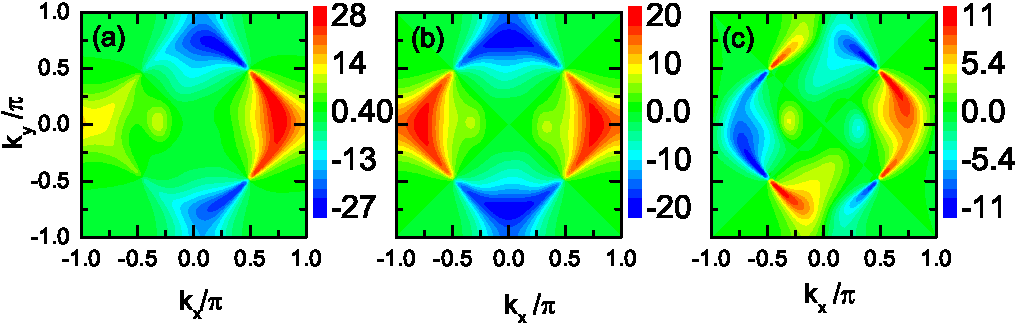
\includegraphics[scale=0.8]{pic/fig22}
\caption{(a)反常格林函数计算轨道1的超导序参量(b)轨道1单重态通道的序参量(c)轨道1三重态通道的序参量}\label{fig21}
\end{figure}
%============================================
\subsection{系统边界处的反常格林函数}
接下来我们利用运动方程来计算系统边界上的反常格林函数,首先从描述2D拓扑绝缘体在圆柱体结构下的哈密顿量开始。通常我们可以将几个哈密顿量进行对角化$H=\sum_n\epsilon_n\gamma^\dagger\gamma$。对2D拓扑绝缘体而言,它的体态始终存在能隙,而低能($\epsilon_n\rightarrow 0$)准粒子激发通常出现在系统的边界上。准粒子算符$\gamma^\dagger$与原来的粒子算符$c_{k_x,\tau\sigma}$之间是通过能量本征值$\epsilon_n$对应的本征矢量联系起来的,利用这个关系我们就可以得到2D拓扑绝缘体在边界上的哈密顿量。在$i_y=1$这个边界上,有效的哈密顿量可以近似的表示为
\begin{equation}
H_{(i_y=1)}=-\sum_{\sigma,\tau}\sigma k c_{k\tau\sigma}^\dagger c_{k\tau\sigma}-\sum_\sigma(\sigma k c_{k1\sigma}^\dagger c_{k2\sigma}+h.c),\label{iy1}
\end{equation}
这里将$k_x$简记为$k$,$\sigma$取$\pm$代表着自旋向上与自旋向下。

高温超导体层的哈密顿量为
\begin{equation}
H_{SC}=\sum_\sigma\epsilon_{k} d_{k\sigma}^\dagger d_{k\sigma}+(\Delta_{ k} d_{k\uparrow}^\dagger d_{-k\downarrow}^\dagger+h.c).
\end{equation}

两层之间的耦合为
\begin{equation}
H_I=-\sum_{\sigma,\tau}(t_\perp c_{k\tau\sigma}^\dagger d_{k\sigma}+h.c).
\end{equation}

为了计算方便,先定义下面的六个格林函数元素
$x_1=\langle\langle c_{k1\uparrow}^\dagger|c_{-k1\downarrow}^\dagger$$\rangle$$\rangle_\omega$, $x_2=\langle\langle c_{k2\uparrow}^\dagger|c_{-k1\downarrow}^\dagger$$\rangle$$\rangle_\omega$, $x_3=\langle\langle d_{k\uparrow}^\dagger|c_{-k1\downarrow}^\dagger\rangle\rangle_\omega$, $x_4=\langle\langle d_{-k\downarrow}|c_{-k1\downarrow}^\dagger\rangle\rangle_\omega$, $x_5=\langle\langle c_{-k1\downarrow}|c_{-k1\downarrow}^\dagger\rangle\rangle_\omega$, $x_6=\langle\langle c_{-k2\downarrow}|c_{-k1\downarrow}^\dagger\rangle\rangle_\omega$,根据运动方程(\ref{gf11})可以得到下面的方程组
\begin{subequations}
	\begin{eqnarray}
	(\omega+k)x_1&=&-kx_2-tx_3\\
	(\omega+k)x_2&=&-kx_1-tx_3\\
	(\omega-\epsilon_{k})x_3&=&-t(x_1+x_2)+\Delta_{k} x_4\\
	(\omega+\epsilon_{k})x_4&=&t(x_5+x_6)+\Delta_{k} x_3\\
	(\omega+k)x_5&=&1-k x_6+tx4\\
	(\omega+k)x_6&=&-k x_5+tx_4
	\end{eqnarray}\label{agf2}
\end{subequations}
通过求解方程组(\ref{agf2})就可以得到边界上轨道1的反常格林函数
\begin{equation}
F_{(i_y=1)}=\frac{\Delta_{k} t_\perp^2}{\Delta_k^2(2k+\omega)^2+\epsilon_k^2(2k+\omega)^2-[-2t_\perp^2+\omega(2k+\omega)]^2}.
\end{equation}

其他边界上的有效哈密顿量同样可以得到
\begin{equation}
H_{(i_y=N_y)}=\sum_{\sigma,\tau}\sigma k c_{k\tau\sigma}^\dagger c_{k\tau\sigma}-\sum_\sigma(\sigma k c_{k1\sigma}^\dagger c_{k2\sigma}+h.c),\label{iyn}
\end{equation}

\begin{equation}
H_{(i_x=1)}=\sum_{\sigma,\tau}\sigma k c_{k\tau\sigma}^\dagger c_{k\tau\sigma}-\sum_\sigma(i k c_{k1\sigma}^\dagger c_{k2\sigma}+h.c),\label{ix1}
\end{equation}

\begin{equation}
H_{(i_x=N_x)}=-\sum_{\sigma,\tau}\sigma k c_{k\tau\sigma}^\dagger c_{k\tau\sigma}-\sum_\sigma(i k c_{k1\sigma}^\dagger c_{k2\sigma}+h.c),\label{ixn}
\end{equation}
利用相似的求解方法,可以得到这些边界上轨道1的反常格林函数为
\begin{equation}
F_{(i_y=N_y)}=\frac{\Delta_k t_\perp^2}{(\Delta_k^2+\epsilon_k^2)\omega^2-(-2t_\perp^2+\omega^2)^2}\label{cyyL}.
\end{equation}

\begin{equation}
F_{(i_x=1)}=-\frac{\Delta_k  t_\perp^2 \left(2 k^2+2 k \omega +\omega ^2\right)}{4 k^2 \left[t_\perp^4-\omega ^2 \left(\Delta_k ^2+2 t_\perp^2+\epsilon_k ^2\right)+\omega ^4\right]+4 k \omega  \left[2 t_\perp^4-\omega ^2 \left(\Delta_k ^2+3 t_\perp^2+\epsilon_k ^2\right)+\omega ^4\right]+4 t_\perp^4 \omega ^2-\omega ^4 \left(\Delta_k ^2+4 t_\perp^2+\epsilon_k ^2\right)+\omega ^6}\label{cyxL}
\end{equation}
	
\begin{equation}
F_{(i_x=N_x)}=-\frac{\Delta_k  t_\perp^2 \left(2 k^2-2 k \omega +\omega ^2\right)}{4 k^2 \left[t_\perp^4-\omega ^2 \left(\Delta_k ^2+2 t_\perp^2+\epsilon_k ^2\right)+\omega ^4\right]-4 k \omega  \left[2 t_\perp^4-\omega ^2 \left(\Delta_k ^2+3 t_\perp^2+\epsilon_k ^2\right)+\omega ^4\right]+4 t_\perp^4 \omega ^2-\omega ^4 \left(\Delta_k ^2+4 t_\perp^2+\epsilon_k ^2\right)+\omega ^6}\label{cyx1}
\end{equation}

在低能量下,对这些反常格林函数做低阶泰勒展开
\begin{equation}
\begin{aligned}
F_{(i_y=1)}\approx&-\frac{\Delta_k  t_\perp^2}{-\Delta_k ^2 \omega ^2+4 t_\perp^4-4 t_\perp^2 \omega ^2+\omega ^4-\omega ^2 \epsilon_k ^2}-\frac{4  \left[\Delta_k  t_\perp^2 \left(\Delta_k ^2 \omega +2 t_\perp^2 \omega -\omega ^3+\omega  \epsilon_k ^2\right)\right]}{\left(-\Delta_k ^2 \omega ^2+4 t_\perp^4-4 t_\perp^2 \omega ^2+\omega ^4-\omega ^2 \epsilon_k ^2\right)^2}k\\
&+\frac{4 \Delta_k   t_\perp^2 \left[-4 t_\perp^4 \left(\Delta_k ^2+\epsilon_k ^2\right)+6 \omega ^4 \left(\Delta_k ^2+2 t_\perp^2+\epsilon_k ^2\right)-3 \omega ^2 \left(\Delta_k ^2+2 t_\perp^2+\epsilon_k ^2\right)^2-3 \omega ^6\right]}{\left(4 t_\perp^4-\omega ^2 \left(\Delta_k ^2+4 t_\perp^2+\epsilon_k ^2\right)+\omega ^4\right)^3}k^2,
\end{aligned}
\end{equation}
\begin{equation}
F_{(i_y=N_y)}=-\frac{\Delta_k  t_\perp^2}{-\Delta_k ^2 \omega ^2+4 t_\perp^4-4 t_\perp^2 \omega ^2+\omega ^4-\omega ^2 \epsilon_k ^2},
\end{equation}



\begin{equation}
\begin{aligned}
&F_{(i_x=1)}\approx-\frac{\Delta_k  t_\perp^2}{-\Delta_k ^2 \omega ^2+4 t_\perp^4-4 t_\perp^2 \omega ^2+\omega ^4-\omega ^2 \epsilon_k ^2}+\frac{2 \Delta_k   t_\perp^2 \omega  \left(\Delta_k ^2+2 t_\perp^2-\omega ^2+\epsilon_k ^2\right)}{\left(-\Delta_k ^2 \omega ^2+4 t_\perp^4-4 t_\perp^2 \omega ^2+\omega ^4-\omega ^2 \epsilon_k ^2\right)^2}k\\
&+\frac{2 \Delta_k   t_\perp^2 \left[-3 \omega ^4 \left(\Delta_k ^2-\omega ^2+\epsilon_k ^2\right)^2-8 t_\perp^8+24 t_\perp^6 \omega ^2+6 t_\perp^4 \omega ^2 \left(\Delta_k ^2-5 \omega ^2+\epsilon_k ^2\right)-16 t_\perp^2 \omega ^4 \left(\Delta_k ^2-\omega ^2+\epsilon_k ^2\right)\right]}{\omega ^2 \left(4 t_\perp^4-\omega ^2 \left(\Delta_k ^2+4 t_\perp^2+\epsilon_k ^2\right)+\omega ^4\right)^3}k^2,
\end{aligned}
\end{equation}
\begin{equation}
\begin{aligned}
&F_{(i_x=N_x)}\approx-\frac{\Delta_k  t_\perp^2}{-\Delta_k ^2 \omega ^2+4 t_\perp^4-4 t_\perp^2 \omega ^2+\omega ^4-\omega ^2 \epsilon_k ^2}-\frac{2  \left(\Delta_k  t_\perp^2 \omega  \left(\Delta_k ^2+2 t_\perp^2-\omega ^2+\epsilon_k ^2\right)\right)}{\left(-\Delta_k ^2 \omega ^2+4 t_\perp^4-4 t_\perp^2 \omega ^2+\omega ^4-\omega ^2 \epsilon_k ^2\right)^2}k\\
&+\frac{2 \Delta_k   t_\perp^2 \left[-3 \omega ^4 \left(\Delta_k ^2-\omega ^2+\epsilon_k ^2\right)^2-8 t_\perp^8+24 t_\perp^6 \omega ^2+6 t_\perp^4 \omega ^2 \left(\Delta_k ^2-5 \omega ^2+\epsilon_k ^2\right)-16 t_\perp^2 \omega ^4 \left(\Delta_k ^2-\omega ^2+\epsilon_k ^2\right)\right]}{\omega ^2 \left(4 t_\perp^4-\omega ^2 \left(\Delta_k ^2+4 t_\perp^2+\epsilon_k ^2\right)+\omega ^4\right)^3}k^2.
\end{aligned}
\end{equation}
这里的$k^2$项是由无能隙的边界态贡献的有效单重态的配对,在$i_x=1$与$i_x=N_x$边界上,反常格林函数在单重态的贡献是完全相同的。然而在$i_y=N_y$边界上,来自轨道内的耦合贡献于轨道间的耦合贡献相互抵消,所以在这个边界上电子有效配对的量值非常小。

上面的结果也可以通过定性的方式进行乐姐,如公式(\ref{iy1},\ref{iyn},\ref{ix1},\ref{ixn})所示,边界有效哈密顿量同时包含了轨道间以及轨道内的跃迁项,当与超导体进行耦合时,这两部分都会对边界上的有效电子配对有贡献。轨道内的跃迁应该与2D拓扑绝缘体螺旋边界态的性质相同,在两个边界上会发生反号。而且从公式(\ref{tiham})中可以看出在$i_y$的边界上,轨道间的跃迁是个实常数,在$i_x$边界上则是虚常数。结果就是在$i_y=N_y$边界上,轨道间的跃迁常数与轨道内的跃迁常数实相反的,它们之间会相互抵消,从而在这个边界上形成的电子配对会非常小。然而在$i_y=1$边界上,这个项的贡献是相同的,会叠加起来,从而在这个边界上的电子配对强度会变得比较大。对于$i_x=1$或者$i_x=N_x$边界,轨道间的跃迁常数是虚常数,在这个边界上同样可以诱导出有效的$d$-波电子配对,但是其大小会小于$i_y=1$边界上。
%============================================
\subsection{本章总结}
在本章中,通过运动方程的方法,我们计算了体态电子的反常格林函数,得到了与数值计算相同的结果,并发现的确会同时存在奇宇称和偶宇称两种不同通道的电子配对。通过近邻效应在拓扑绝缘体中会同时诱导处$d$-波电子配对和$p$-波电子配对。而$p$-波配对则主要是来源于拓扑绝缘体中自旋轨道耦合的贡献。

接下俩我们利用边界有效的哈密顿量,利用运动方程对每个边界上的反常格林函数进行了计算,结果发现在不同边界上诱导出的电子配对形式是不相同的,特别是在$i_y=N_y$这个边界上,因为自旋轨道耦合的作用,这条边界上的电子配对会非常小,从而使得2D拓扑绝缘体的螺旋边界态始终未能打开能隙,而其它三个边界上都会存在可观大小的$d$-波电子配对。这也成功的解释了为何在体系中,与上边界相邻的位置无法产生马约拉纳拐角态。












